\documentclass[a4paper,twoside,11pt]{article}
\usepackage{a4wide,graphicx,fancyhdr,amsmath,amssymb,float}
\usepackage{algorithmic}
\usepackage{hyperref}
\usepackage{url}

%----------------------- Macros and Definitions --------------------------

\setlength\headheight{20pt}
\addtolength\topmargin{-10pt}
\addtolength\footskip{20pt}

\newcommand{\N}{\mathbb{N}}
\newcommand{\ch}{\mathcal{CH}}
\everymath{\displaystyle}
\newcommand{\solution}[1]{\noindent{\bf Solution to Exercise #1:}}

\fancypagestyle{plain}{%
\fancyhf{}
\fancyhead[LO,RE]{\sffamily\bfseries\large Technische universiteit Eindhoven}
\fancyhead[RO,LE]{\sffamily\bfseries\large 2IV35 Visualization}
\fancyfoot[LO,RE]{\sffamily\bfseries\large department of mathematics and computer science}
\fancyfoot[RO,LE]{\sffamily\bfseries\thepage}
\renewcommand{\headrulewidth}{0pt}
\renewcommand{\footrulewidth}{0pt}
}

\pagestyle{fancy}
\fancyhf{}
\fancyhead[RO,LE]{\sffamily\bfseries\large Technische universiteit Eindhoven}
\fancyhead[LO,RE]{\sffamily\bfseries\large 2IV35 Visualization}
\fancyfoot[LO,RE]{\sffamily\bfseries\large department of mathematics and computer science}
\fancyfoot[RO,LE]{\sffamily\bfseries\thepage}
\renewcommand{\headrulewidth}{1pt}
\renewcommand{\footrulewidth}{0pt}

%-------------------------------- Title ----------------------------------

\title{\vspace{-\baselineskip}\sffamily\bfseries 2IV35 Visualization Set 2}
\author{Jeroen van Oorschot \qquad Student number: 0721913 \\{\tt j.v.oorschot@student.tue.nl}\\ \\Mart Pluijmaekers \qquad Student number: 0753117 \\{\tt m.h.l.pluijmaekers@student.tue.nl}}

\date{\today}

%--------------------------------- Text ----------------------------------

\begin{document}
\maketitle

\pagebreak
\tableofcontents
\newpage
\section{Volume Rendering}
\subsection{Tri-linear interpolation}
To make sure we can also get data from between points we want to do some interpolation on the data. So we use the following function to get a value on point $(x,y,z)$ in a field $F$ with the value $F[i][j][k]$ for the integer values $i$, $j$ and $k$ by calculating the value $val$ with:
\begin{eqnarray*}
\alpha =& x-\lfloor x \rfloor\\
\beta =& y-\lfloor y \rfloor\\
\gamma =& z-\lfloor z \rfloor\\
val =& (1 - \alpha) * (1 - \beta) * (1 - \gamma ) * F[\lfloor x \rfloor][\lfloor y \rfloor][\lfloor z \rfloor] \\
&+ \alpha * (1 - \beta) * (1 - \gamma ) * F[\lceil x \rceil][\lfloor y \rfloor][\lfloor z \rfloor]\\
                    &+ (1 - \alpha) * \beta * (1 - \gamma ) * F[\lfloor x \rfloor][\lceil y \rceil][\lfloor z \rfloor] \\
                    &+ \alpha * \beta * (1 - \gamma ) * F[\lceil x \rceil][\lceil y \rceil][\lfloor z \rfloor]\\
                    &+ (1 - \alpha) * (1 - \beta) * \gamma  * F[\lfloor x \rfloor][\lfloor y \rfloor][\lceil z \rceil] \\
                    &+ \alpha * (1 - \beta) * \gamma  * F[\lceil x \rceil][\lfloor y \rfloor][\lceil z \rceil]\\
                    &+ (1 - \alpha) * \beta * \gamma  * F[\lfloor x \rfloor][\lceil y \rceil][\lceil z \rceil] \\
                    &+ \alpha * \beta * \gamma  * F[\lceil x \rceil][\lceil y \rceil][\lceil z \rceil]
\end{eqnarray*}
\subsection{Gaining speed}
We implemented two ways to speed up the program, one is by making a low and a high resolution maximum intensity projection(MIP), in the lower resolution version (simply called MIP) we start at one and take steps of two in calculating pixel colour, while setting pixels $(x,y)$,$(x-1,y)$,$(x,y-1)$ and $(x-1,y-1)$ to that color. We also added the option to manually adjust the number of samples. Results of tests on the backpack dataset can be found in this table, the numbers represent the rendering time in ms:
\begin{center}
  \begin{tabular}{| l || r | r | }
    \hline
    samples & hi & low \\ \hline
    223 & 11904 & 2933 \\ \hline
    22 & 1280 & 372 \\
    \hline
  \end{tabular}
\end{center}

\section{Maximum intensity projection}
In maximum intensity projection (MIP) we traverse trough the data and project at the point where that ray hits the screen the maximum of the samples on that ray. After implementing maximum intensity projection we opened all data sets with to get the following results.
\subsection{Backpack}
This worked fine, it was easy to see there were objects resembling a bullet, a drug needle, a Swiss army knife and a spray can in the backpack, so this technique would be suitable on an airport, because we can pick out the backs worth examining. Without rotating the data the contents can be obscured, but after rotating you could get to see everything clearly as can be seen in Figure \ref{MB}.
\begin{figure}[!h]
  \centering
  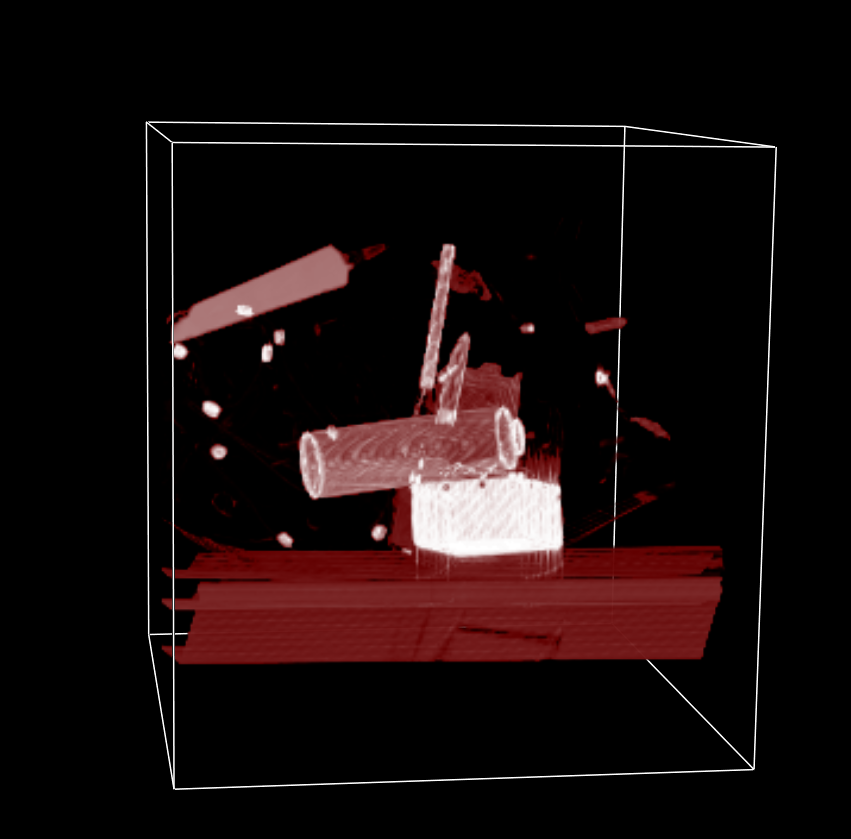
\includegraphics[width=0.5\textwidth]{MB.png}
  \caption{Resulting picture for backpack with MIP}
  \label{MB}
\end{figure}
\subsection{Bonsai}
This worked fine, we could see there was a tree. A picture is included in Figure \ref{MBon}.
\begin{figure}[!h]
  \centering
  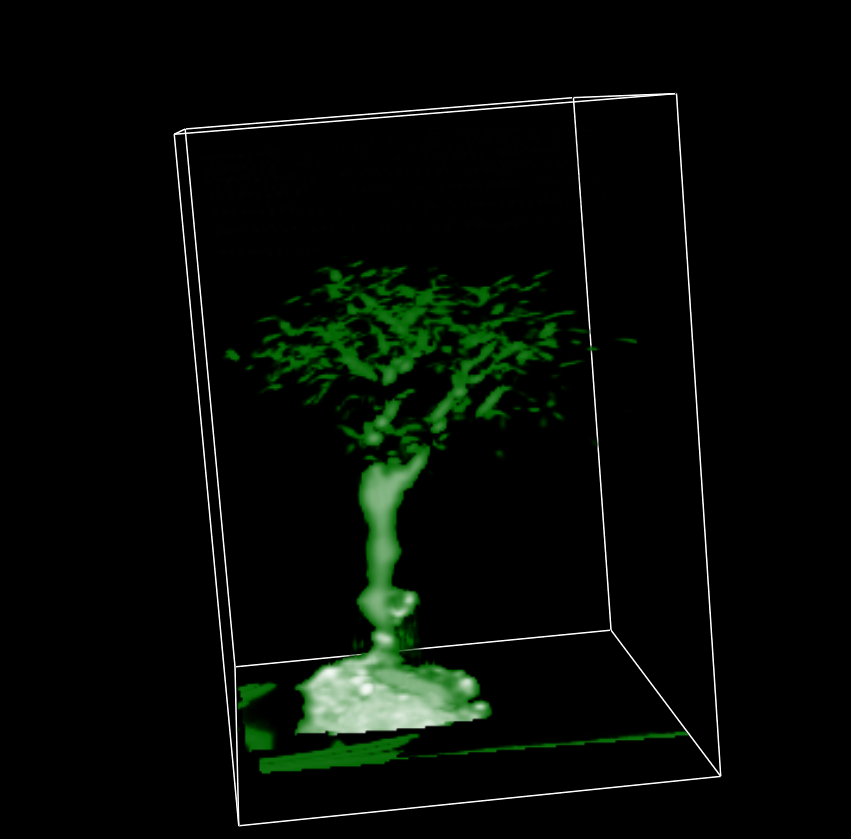
\includegraphics[width=0.5\textwidth]{MBon.png}
  \caption{Resulting picture for Bonsai with MIP}
  \label{MBon}
\end{figure}
\subsection{Carp}
This worked fantastic, we could see all the bones in the carp. A picture of the tail is included in Figure \ref{MCT}, the side is in Figure \ref{MCS}.
\begin{figure}[!h]
  \centering
  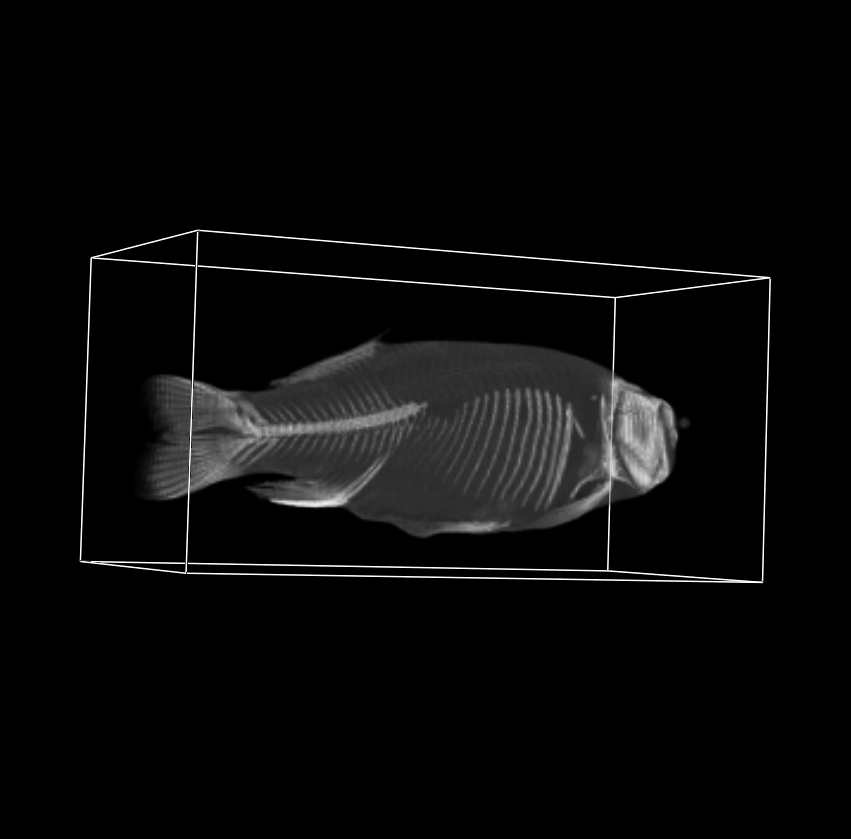
\includegraphics[width=0.5\textwidth]{MCT.png}
  \caption{Resulting picture for tail of the carp with MIP}
  \label{MCT}
\end{figure}
\begin{figure}[!h]
  \centering
  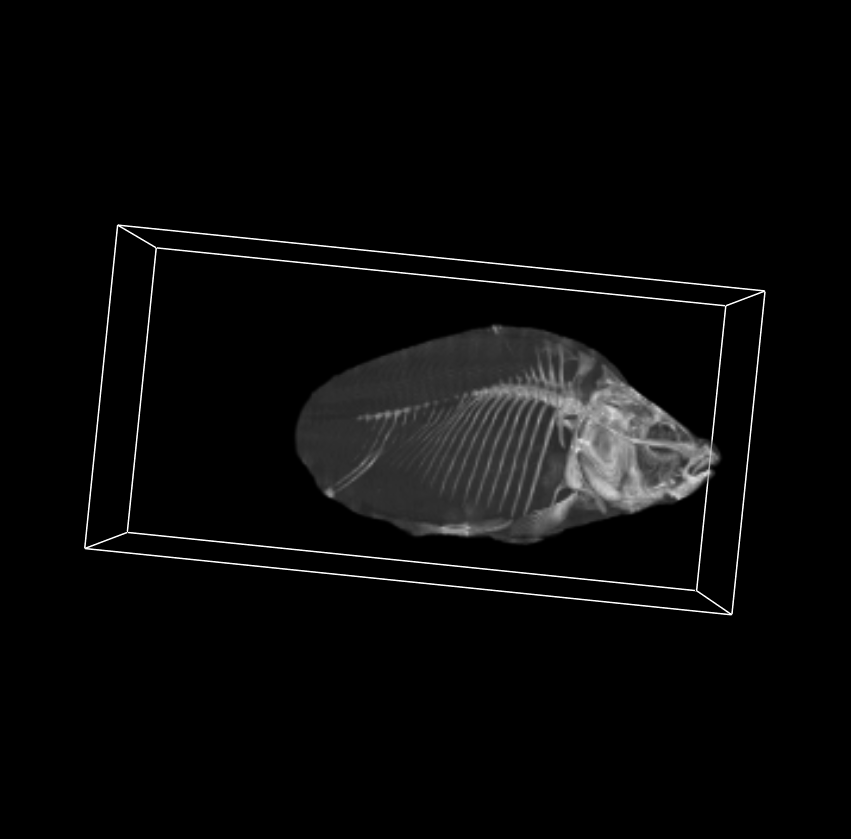
\includegraphics[width=0.5\textwidth]{MCS.png}
  \caption{Resulting picture for side of the carp with MIP}
  \label{MCS}
\end{figure}

\subsection{Orange}
This dataset leant itself to MIP too, we even were able to give the peel an orange color, while giving the inside a blue color. A picture is included in Figure \ref{MO}.
\begin{figure}[!h]
  \centering
  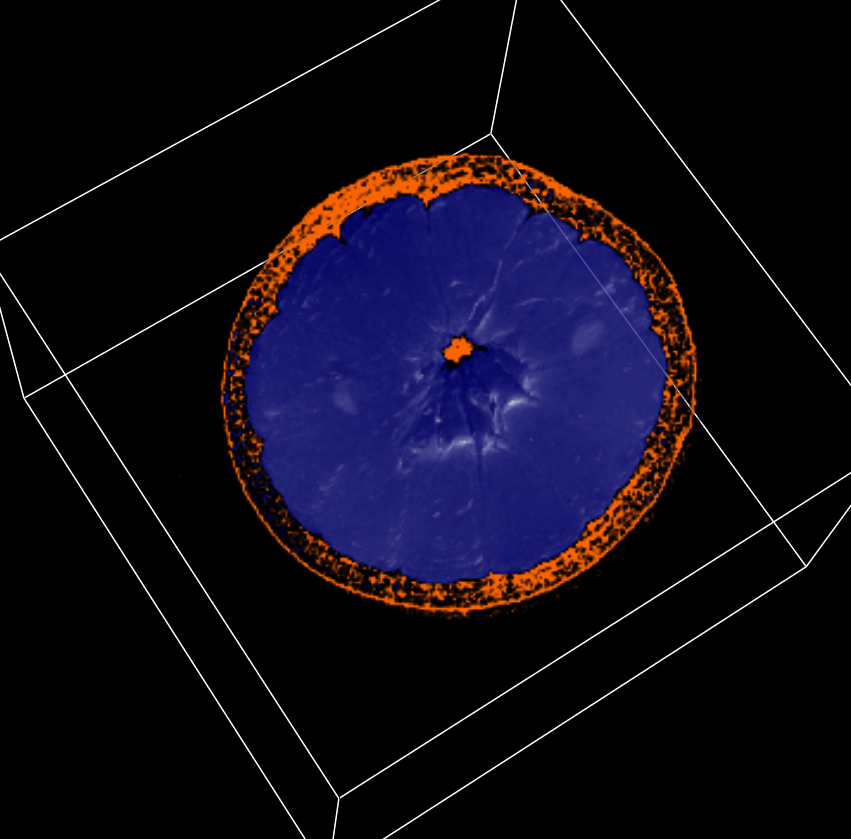
\includegraphics[width=0.5\textwidth]{MO.png}
  \caption{Resulting picture for orange with MIP}
  \label{MO}
\end{figure}

\subsection{Pig}
In this example we were able so show the coins in yellow and the pig in pink, also the hole is visible. A picture is included in Figure \ref{MP}.
\begin{figure}[!h]
  \centering
  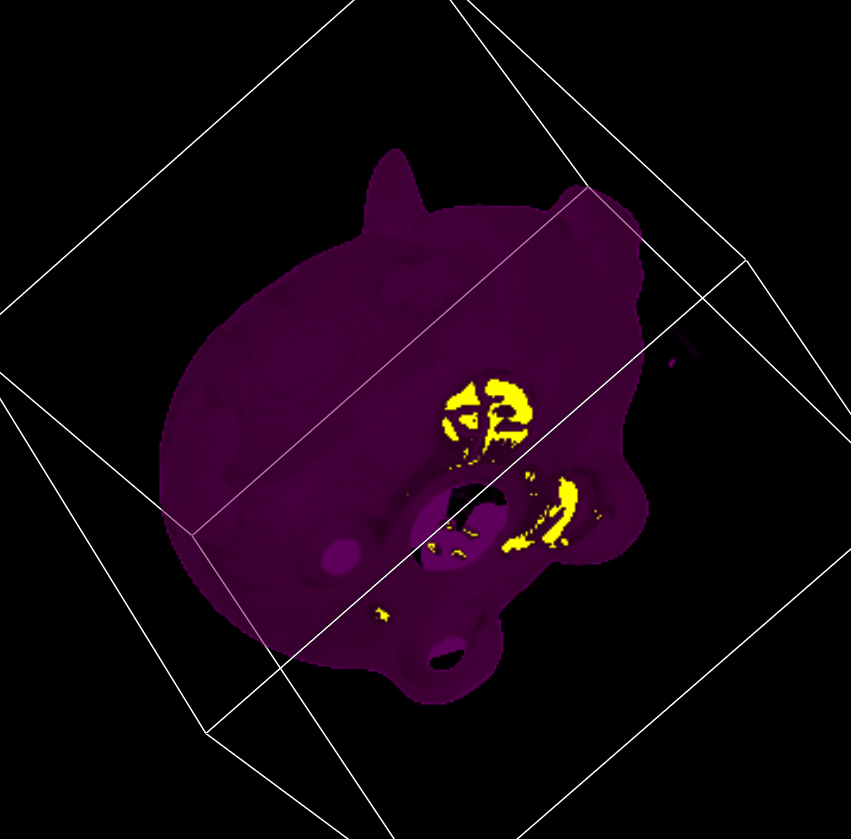
\includegraphics[width=0.5\textwidth]{MP.png}
  \caption{Resulting picture for pig with MIP}
  \label{MP}
\end{figure}

\subsection{Human}
Again a clear picture of a skeleton. A picture is included in Figure \ref{MH}.
\begin{figure}[!h]
  \centering
  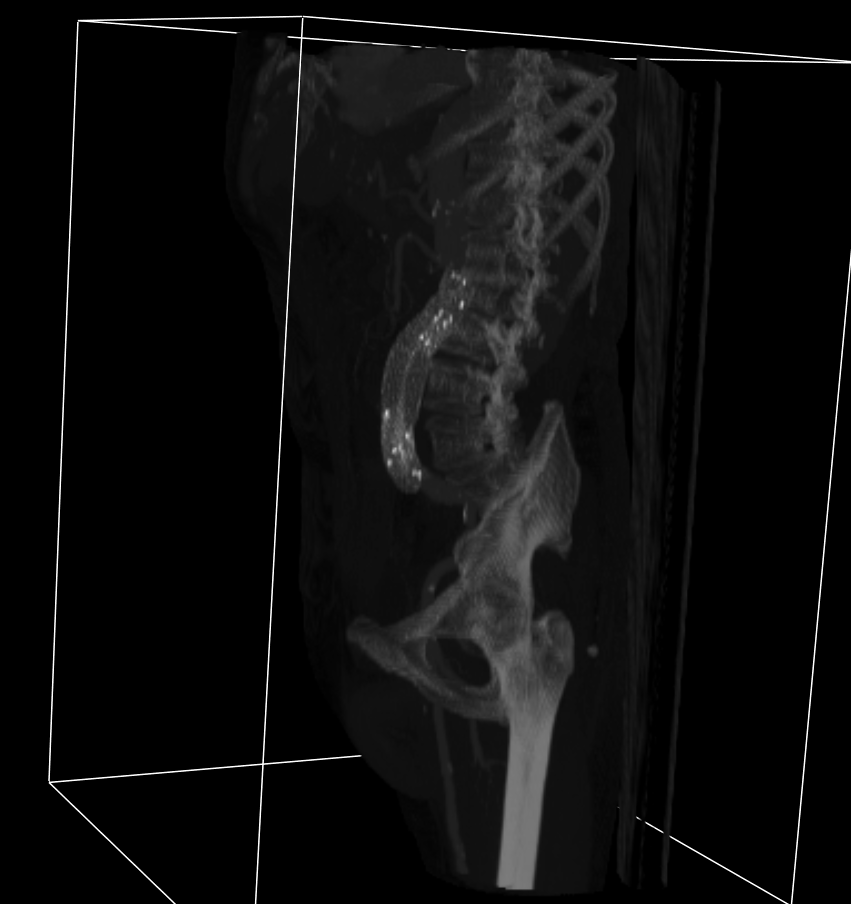
\includegraphics[width=0.5\textwidth]{MH.png}
  \caption{Resulting picture for human with MIP}
  \label{MH}
\end{figure}

\subsection{Tomato}
The tomato did not look very good as a picture because its quite homogeneous and quite similar to the orange, therefor we decided to omit a picture of it.

\subsection{Tooth}
The tooth data also produced nice results as can be seen in Figure \ref{MT}.
\begin{figure}[!h]
  \centering
  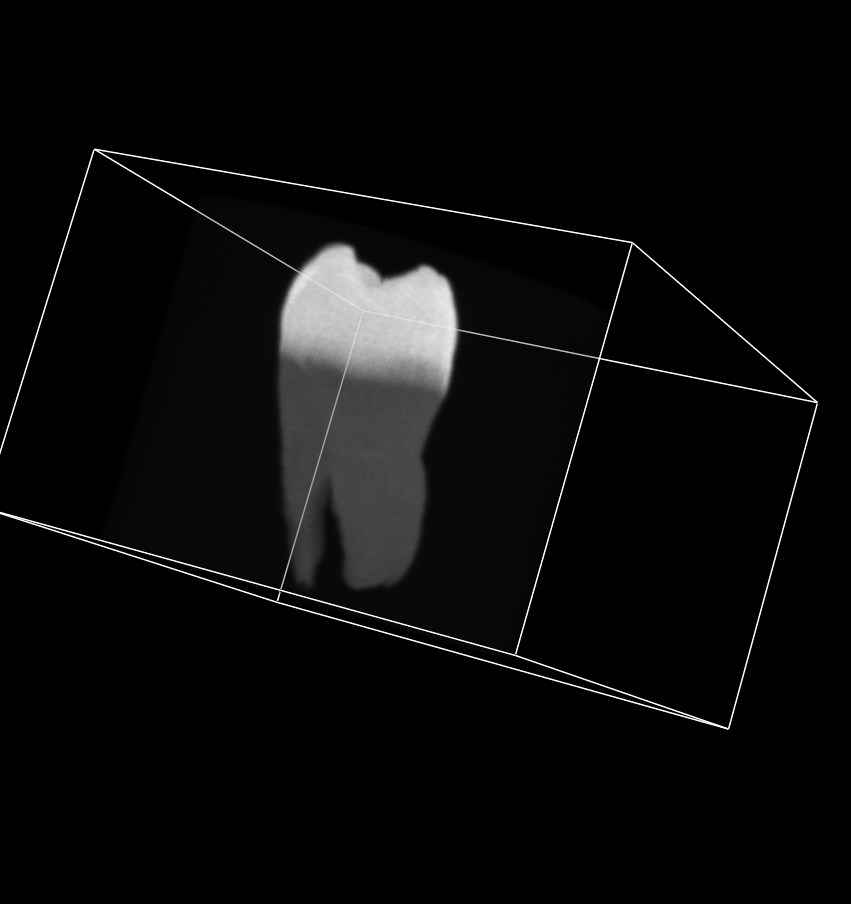
\includegraphics[width=0.5\textwidth]{MT.png}
  \caption{Resulting picture for tooth with MIP}
  \label{MT}
\end{figure}


 
 \section{Compositing}
 For compositing we implemented the standard formula given in slides of the course 2IV35 (Visualization) of the TU/e \cite{slideVis_m}. Compositing is a process where the values of all voxels along the ray are merged in such a way that one should be able to also look at the insides, where masses which are big will have a heavier impact on the picture then smaller masses. This can be remedied by setting the transfer function carefully but it could be that the transferfunction needs to be readjusted after rotating the picture, since now the ray has to traverse more or less of the material then it did previously.
 
 \subsection{Backpack}
 For the backpack data we also tried to get the backpack itself visible, unfortunately it did not work the way we intended. We can now estimate the shape of the backpack, but can still not see the bag itself or atleast not in a clear manner.
 
 \begin{figure}[h]
 \centering
 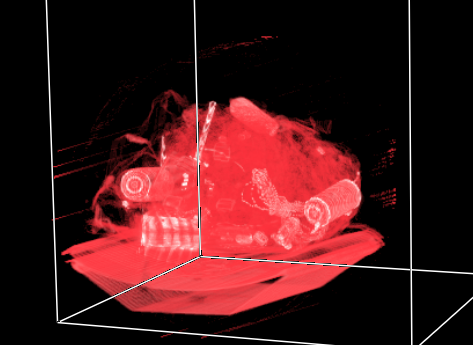
\includegraphics[scale=0.7]{images/backpackComp}
 \caption{Backpack view of both contents and outside}
 \label{backpackComp}
 \end{figure}
 
 \subsection{Bonsai}
 Using composition we managed to get a better view of the form of the bonsai tree then was possible with MIP since now the entire ray was taken into account. Note that the leaves are not shown. Of the stem however, we see a much more defined shape and higher level of detail.
 
  \begin{figure}[h]
 \centering
 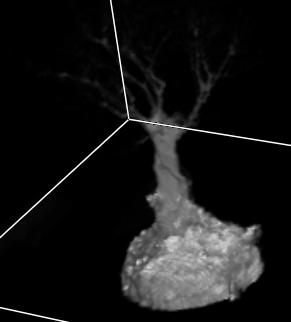
\includegraphics[scale=0.7]{images/bonsaiComp2}
 \caption{Better defined shape of the bonsai}
 \label{bonsaiComp2}
 \end{figure}
 
 
 \subsection{Carp}
 Using compositing we can again see some more detail in the carp. Not only can we see the densest bits, we can also see the less dense parts of the carp which are also used for its movements, like the backfins as can be seen in figure \ref{carpComp3}. Also the outside can be more defined as can be seen in figure \ref{carpComp}. Furthremore since we now can look ``inside'' the carp we can see there is some form of cavity within the carp as can be seen in figure \ref{carpComp2}.
 
 \begin{figure}[h]
  \minipage{0.32\textwidth}
 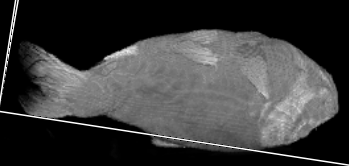
\includegraphics[width=\linewidth]{images/carpComp}
 \caption{Outline of the carp.}
 \label{carpComp}
\endminipage\hfill
\minipage{0.32\textwidth}
 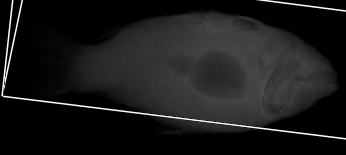
\includegraphics[width=\linewidth]{images/carpComp2}
 \caption{Cavity within the carp}
 \label{carpComp2}
\endminipage\hfill
\minipage{0.32\textwidth}
 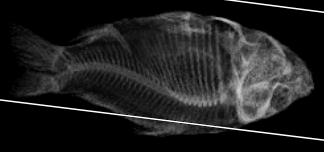
\includegraphics[width=\linewidth]{images/carpComp4}
 \caption{Structural parts of the carp}
 \label{carpComp3}
\endminipage\hfill
 \centering
 \end{figure}
 
 \subsection{Orange}
 Using compositing we can visualize the outline of the orange perfectely, something which is not possible with using MIP (figure \ref{orangeComp}), furthermore we can also use it to make the interiors more visible as can be seen in figure \ref{orangeCompOp}.

 \begin{figure}[h]
 \centering
 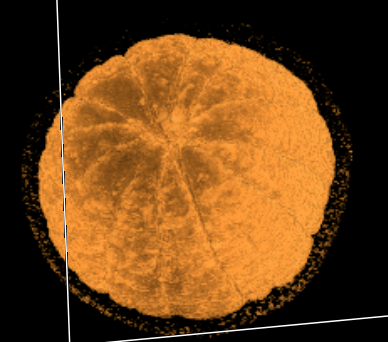
\includegraphics[scale=0.7]{images/orangeComp}
 \caption{Orange using compositing}
 \label{orangeComp}
  \end{figure} 
 
 \subsection{Pig}
 It now becomes aparent that the pig dataset is not a scan of a pig, but of a piggy bank. Furthermore we can clearly see that there are some flowers on the outside and that it should be opened from the bottom (figure \ref{pigComp}), it also has some coins in its interior, which could be studied better using opacity weighting (figure \ref{pigComp2}).
 
   \begin{figure}[H]
 \minipage{0.4\textwidth}
  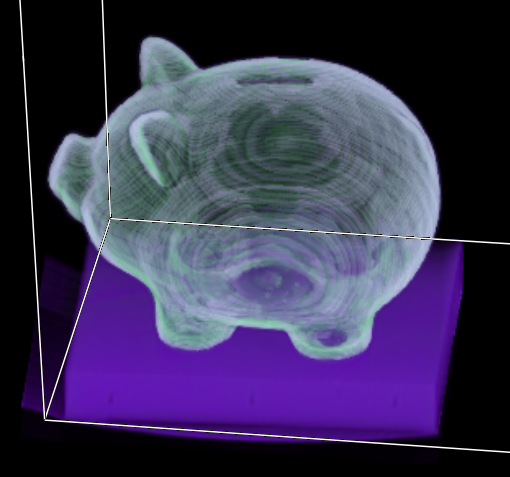
\includegraphics[width=\linewidth]{images/pigComp}
  \caption{Piggybank with one of the flowers and the bottom opening visible}\label{pigComp}
\endminipage\hfill
\minipage{0.5\textwidth}
  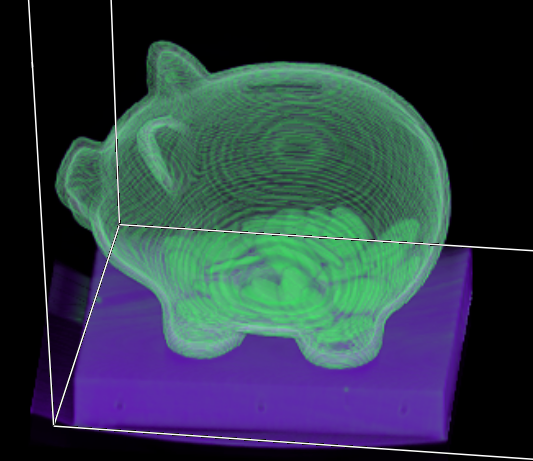
\includegraphics[width=\linewidth]{images/pigComp2}
  \caption{Piggybank with the coins visible}\label{pigComp2}
\endminipage\hfill
 \end{figure}
 
 \subsection{Human}
 From the MIP we could see the skeleton quite clearly, but the skin was lacking, since bone is much more dense than skin. Compositing however can make skin visible as can be seen in figure \ref{bodyComp}. While also making bones visible as can be seen in figure \ref{bodyComp2}.
    \begin{figure}[H]
 \minipage{0.4\textwidth}
  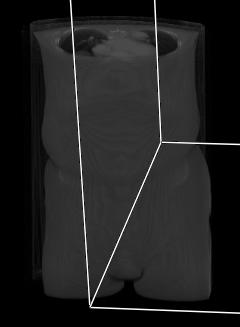
\includegraphics[width=\linewidth]{images/bodyComp}
  \caption{Sking of the torso with some bones at the top}\label{bodyComp}
\endminipage\hfill
\minipage{0.5\textwidth}
  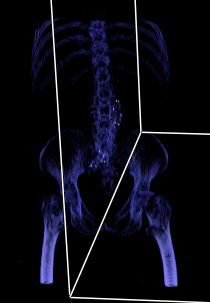
\includegraphics[width=\linewidth]{images/bodyComp2}
  \caption{Only the skeleton of the torso}\label{bodyComp2}
\endminipage\hfill
 \end{figure}
 
 
 \subsection{Tomato}
 Since the tomato is too homogeneous for the MIP to see something, we can use it when compositing to atleast get the total shape of the tomato, from which we can see that it is a tomato which has no leaves or stem at the top anymore as can be seen in figure \ref{tomatoComp}.
 
  \begin{figure}[h]
 \centering
 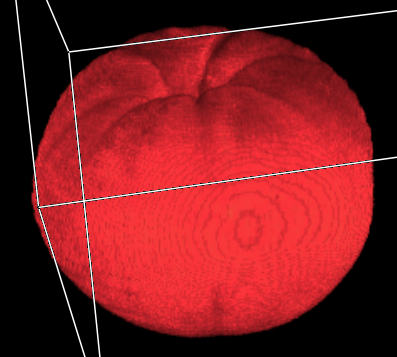
\includegraphics[scale=0.5]{images/tomatoComp}
 \caption{Tomato using compositing}
 \label{tomatoComp}
  \end{figure} 
 
 \subsection{Tooth}
 The tooth for compositing is quite similar to the tooth when doing MIP, we can however make the inside of the tooth visible (the root), but does not produce very solid visualizations since the parameters need to be tweaked in order to keep a consistent picture. We can however see the tooth clearly and that it has 3 legs, as can be seen in figure \ref{toothComp}
 
   \begin{figure}[h]
 \centering
 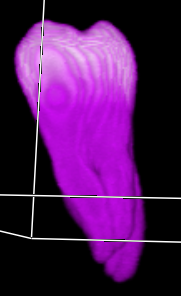
\includegraphics[scale=0.5]{images/toothComp}
 \caption{Tooth using compositing}
 \label{toothComp}
  \end{figure} 
 
 \newpage
 \section{Opacity weighting}
 Opacity weighting is implemented as discribed in a paper by Marc Levoy \cite{levoy_m}. Since there is a need for scaling the gradient magnitude, we implemented a scaling factor using a spinner, which can be used to scale the magnitude. We decided to use this method since it enables a person to have granulated control of the scaling which enables the selection of optimal values for making the borders visible. Opacity weighting remedies the problem of compositing since it voxels which define edges will be made much more visible then voxels in the middle of (homogenuous) masses. This enables more precise viewing of contents of volumes. \\
 
In our program, the transfer function editor can be used to select the regions, every odd point on the transfer function is assumed to be defining a region and its value and opacity are taken from the selected values in the transferfunction editor.
 
 \subsection{Backpack}

  We've taken the backpack data and tried to get a better overview of the backpack itself and the contents of the containers within it too. Using opacity weighting it is much easier to do these things since large (homogeneous) masses do not show up as such. Using these we can see that there is some fabric like contents in the backpack but also that some of the containers are not empty. The images generated can be seen in figures \ref{backpackOp} and \ref{backpackOp2}\\
 
  \begin{figure}[H]
 \minipage{0.4\textwidth}
  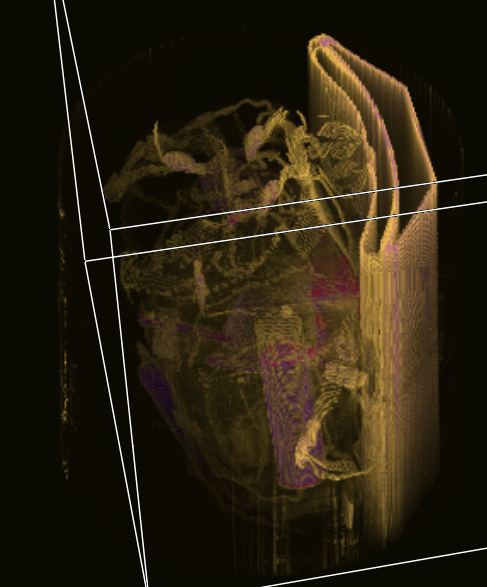
\includegraphics[width=\linewidth]{images/backpackOp}
  \caption{Backpack similar to composition}\label{backpackOp}
\endminipage\hfill
\minipage{0.5\textwidth}
  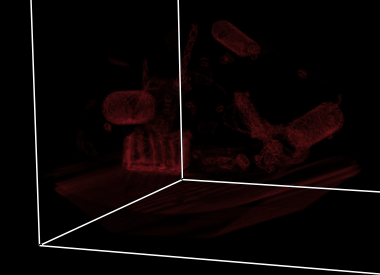
\includegraphics[width=\linewidth]{images/backpackOp2}
  \caption{Backpack with a look into the contents}\label{backpackOp2}
\endminipage\hfill
 \end{figure}
 
 \subsection{Bonsai}
 For the bonsai tree we tried to see if there was some more more present which we could show. There appears to be an oddly shaped container around the bonsai tree which resembles a house. We assume this is the edge of the scan area. The image is displayed in figure \ref{bonsaiOp}
  \begin{figure}[h]
 \centering
 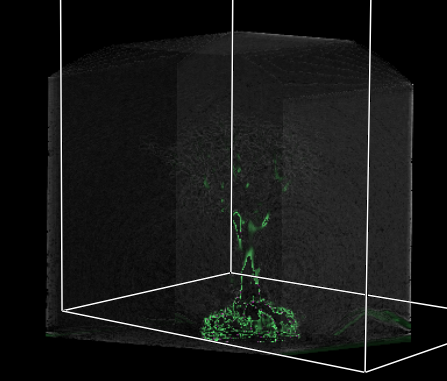
\includegraphics[scale=0.6]{images/bonsaiOp}
 \caption{The bonsai with the protective covering slightly visible}
 \label{bonsaiOp}
 \end{figure}
 
 \subsection{Carp}
 When we applied opacity weighting to the carp dataset we could very quickly see that the carp was laid flat on some sheets which is presumable paper (as can be seen in figure \ref{carpOp}). The head of the fish can be studied quite well since its edges can be clearly marked from the other parts of the body. By scaling back the opacity given to the meat of the fish, the bone structure could be studied too, but since this can be done with MIP too we did not find this very relevant. However, using the same technique, the exact structure of the fish can be studied in more detail.
 \begin{figure}[h]
 \centering
 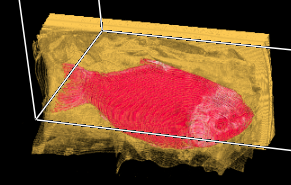
\includegraphics{images/carpOp}
 \caption{The carp with the protective surface visible}
 \label{carpOp}
 \end{figure}
 
 \subsection{Orange}
 Using Compositing we already found out what the shape of the orange actually is, but now we can see both the external shape and the internal sturcture, which reveals some seeds even better then compositing could.  The orange is displayed in figures \ref{orangeOp} and \ref{orangeCompOp}
 \begin{figure}[H]
  \minipage{0.4\textwidth}
 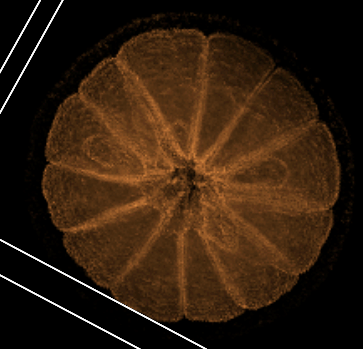
\includegraphics[scale=0.5]{images/orangeOp}
 \caption{Orange with clear seeds and clear outline of the flesh.}
 \label{orangeOp}
\endminipage\hfill
\minipage{0.5\textwidth}
 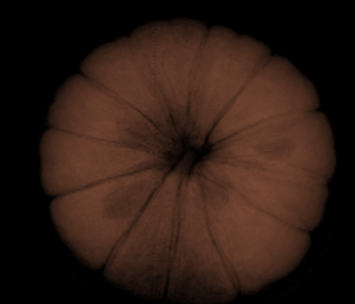
\includegraphics[scale=0.5]{images/orangeCompOp}
 \caption{Same visualization, but using composition}
 \label{orangeCompOp}
\endminipage\hfill
 \centering

 \end{figure}
 
 \subsection{Pig}
 As we saw in the previous section, in the bottom of the piggy bank we have some coins. We've tried to make them more visible, using some more adjustments to the parameters it is possible to get even clearer results. Note that there appear to be harder sections in block at the base of the piggy bank. Since we assume the piggy bank has to be opened from the bottom, we speculate that this is a simple board used to make the surface flat and these spots are remnants of attachment points for that specific board.
 \begin{figure}[H]
 \centering
 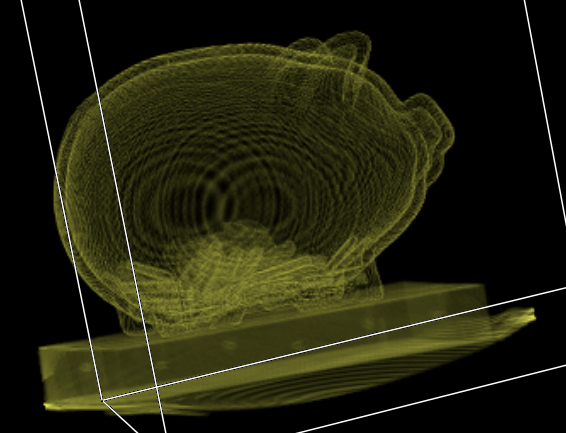
\includegraphics[scale=0.5]{images/pigOp}
 \caption{The piggybank with the coin contents made visible}
 \label{pigOp}
 \end{figure}
 
 \subsection{Human}
 For the human we tried to combine both the outline and the skeleton as can be see in figure \ref{bodyOp} Note that the outline of the skin is very faint in that image. This enables the physician to see where the bones are located relative to the skin.
 \begin{figure}[H]
 \centering
 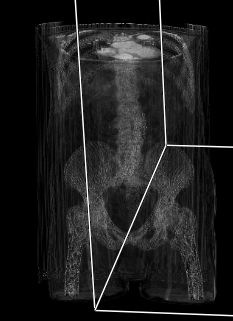
\includegraphics[scale=0.9]{images/bodyOp2}
 \caption{Human torso, with skeleton and skin}
 \label{bodyOp}
 \end{figure}
 
 \subsection{Tomato}
 Usin opacity weighting we tried to get some more specialized pictures of the tomato, we got one where the fleshy bits are shown with the skin, one which only houses the fleshy parts and one which also shows some of the seeds within the tomato. The tomato images are displayed in figures \ref{tomatoOp}, \ref{tomatoOp2} and \ref{tomatoOp3}
 \begin{figure}[htb]
\minipage{0.32\textwidth}
  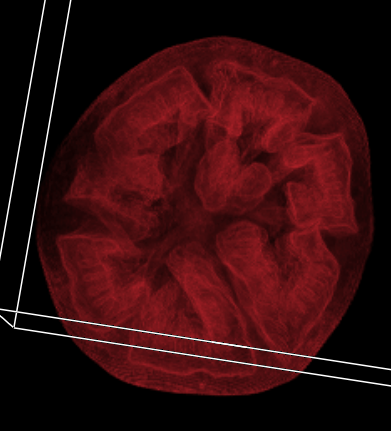
\includegraphics[width=\linewidth]{images/tomatoOp}
  \caption{Mixture of the pulp, the skind and water}\label{tomatoOp}
\endminipage\hfill
\minipage{0.32\textwidth}
  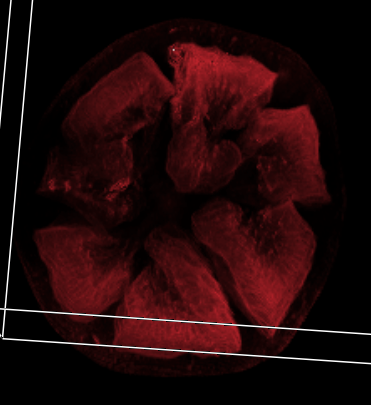
\includegraphics[width=\linewidth]{images/tomatoOp2}
  \caption{Only the pulp visible.}\label{tomatoOp2}
\endminipage\hfill
\minipage{0.32\textwidth}%
  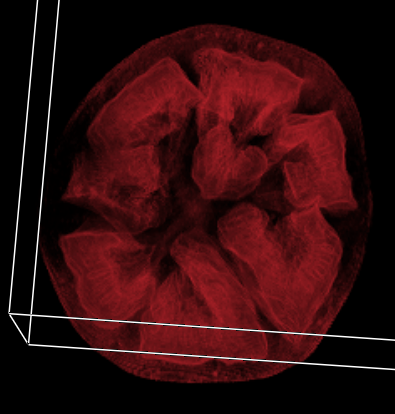
\includegraphics[width=\linewidth]{images/tomatoOp3}
  \caption{Tomato with some seeds visible}\label{tomatoOp3}
\endminipage
\end{figure}

 
 \subsection{Tooth}
 Using compositing we could get the root of the tooth to show, but this was not very clear. Displayed in figures \ref{toothOp} ad \ref{toothOp2} we have a more clear view of the root.
 \begin{figure}[H]
 
 \minipage{0.4\textwidth}
  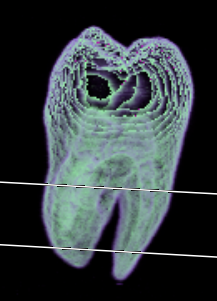
\includegraphics[width=\linewidth]{images/toothOp}
  \caption{The tooth with the root}\label{toothOp}
\endminipage\hfill
\minipage{0.5\textwidth}
  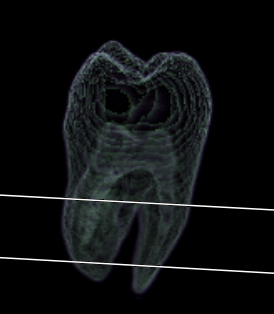
\includegraphics[width=\linewidth]{images/toothOp2}
  \caption{Tooth with a more visible root}\label{toothOp2}
\endminipage\hfill
 \end{figure}


\begin{thebibliography}{9}
\bibitem{slideVis_m}
https://dlwpswbsp.tue.nl/120-2014/4d0982b89c664c579bd307b3c4ae82ca/Slides/4-spatial.pdf
\bibitem{levoy_m}
https://graphics.stanford.edu/papers/volume-cga88/volume.pdf
 \end{thebibliography}
\end{document}
